% !TEX root = ../tex/6-2.tex
% 第6章：本文は青、補足は緑
\newcommand{\asmain}{%
    \setbeamercolor{frametitle}{fg=white,bg=main}%
    \setbeamercolor{structure}{fg=main}%
    \setbeamercolor{itemize item}{fg=main}%
    \setbeamercolor{itemize subitem}{fg=main}%
    \setbeamercolor{enumerate item}{fg=main}%
}
\newcommand{\assuppl}{%
    \setbeamercolor{frametitle}{fg=white,bg=examplecol}%
    \setbeamercolor{structure}{fg=examplecol}%
    \setbeamercolor{itemize item}{fg=examplecol}%
    \setbeamercolor{itemize subitem}{fg=examplecol}%
    \setbeamercolor{enumerate item}{fg=examplecol}%
}
% フレームタイトルの「補足」だけを□で囲む
\newcommand{\supplmark}{%
    \setlength{\fboxsep}{1.5pt}%
    \setlength{\fboxrule}{0.7pt}%
    \fbox{\textbf{補足}}%
}
\asmain


%=============================================
\begin{frame}{6.1から6.2へ}
    \begin{block}{ここまで（6.1）}
        変分／スコア／フローの周辺目標は、$\vx_0$条件付けでtractableになる。\\
        条件付き版は定数差で同値（$J_{\mathrm{CKL}}$／$J_{\mathrm{DSM}}$／$J_{\mathrm{CFM}}$）。
    \end{block}
    \begin{block}{ここから（6.2）}
        予測型を4つに広げ、訓練損失の設計を分解する。\\
        「何が再パラメータ化で、何が最適化に効くか」を整理する。
    \end{block}
\end{frame}
%=============================================
\asmain
\begin{frame}{6.2 の位置づけ}
    \begin{block}{この節の役割}
        拡散の訓練損失を、見通しのよい設計空間として書く
    \end{block}
    \begin{enumerate}
        \item \textbf{6.2.1 四つのパラメータ化}\\
        clean $x$／noise $\veps$／score $s$／velocity $\bm{v}$
        \item \textbf{6.2.2 目的関数の分解}\\
        スケジュール・予測対象・$p_{\mathrm{time}}$・重み$\omega(t)$
        \item \textbf{再パラメータ化 vs 最適化}\\
        代数的同値と、実務で効く違いを区別する
    \end{enumerate}
\end{frame}
%=============================================
\section{6.2.1 四つのパラメータ化}
\asmain
\begin{frame}{区切り：6.2.1 四つのパラメータ化}
    \tableofcontents[currentsection]
\end{frame}
%=============================================
\asmain
\begin{frame}{前向き核の共通設定}
    本節では、特に断らない限り
    \[
        p_t(\vx_t|\vx_0)
        =
        \mathcal{N}(\vx_t;\alpha_t\vx_0,\sigma_t^{2}\bm{I}),
        \qquad
        \vx_0\sim p_{\mathrm{data}}
    \]
    （式4.5.1）を用いる。
    \begin{itemize}
        \item 正の時間重み$\omega:[0,T]\to\mathbb{R}_{>0}$を置く
        \item 4つの標準パラメータ化：$\veps_\phi$、$x_\phi$、$s_\phi$、$\bm{v}_\phi$
        \item 対応する最小化子：$\veps^\star$、$x^\star$、$s^\star$、$\bm{v}^\star$
    \end{itemize}
\end{frame}
%=============================================
\asmain
\begin{frame}{変分視点：何を予測するか}
    DDPM系のKL（2.2.4節、4.5.2節）は、次のどちらかに落ちる：
    \begin{itemize}
        \item $\vx_t$を作ったノイズの期待値（$\veps$-prediction）
        \item $\vx_t$の元になったきれいな信号の期待値（$x$-prediction）
    \end{itemize}
    \begin{block}{見方}
        どちらも「ノイズ観測$\vx_t$から見た条件付き期待」である。\\
        式(6.1.1)の事後平均と同じ思想。
    \end{block}
\end{frame}
%=============================================
\asmain
\begin{frame}{$\veps$-prediction（ノイズ予測）}
    \[
        \veps_\phi(\vx_t,t)
        \approx
        \mathbb{E}[\veps|\vx_t]
        =
        \veps^\star(\vx_t,t)
        \tag{6.2.1}
    \]
    訓練目的：
    \[
        L_{\mathrm{noise}}(\phi)
        :=
        \mathbb{E}_{t}\,
        \omega(t)\,
        \mathbb{E}_{\vx_0,\veps}
        \bigl\|
        \veps_\phi(\vx_t,t)-\veps
        \bigr\|_{2}^{2}
    \]
    \begin{exampleblock}{意味}
        $\veps^\star$は、与えられた$\vx_t$を得るために注入されたノイズの平均。
    \end{exampleblock}
\end{frame}
%=============================================
\asmain
\begin{frame}{$x$-prediction（クリーン予測）}
    \[
        x_\phi(\vx_t,t)
        \approx
        \mathbb{E}[\vx_0|\vx_t]
        =
        x^\star(\vx_t,t)
        \tag{6.2.2}
    \]
    訓練目的：
    \[
        L_{\mathrm{clean}}(\phi)
        :=
        \mathbb{E}_{t}\,
        \omega(t)\,
        \mathbb{E}_{\vx_0,\veps}
        \bigl\|
        x_\phi(\vx_t,t)-\vx_0
        \bigr\|_{2}^{2}
    \]
    \begin{exampleblock}{意味}
        $x^\star$は、ノイズ観測$\vx_t$から見た、あり得るきれいなデータの平均。
    \end{exampleblock}
\end{frame}
%=============================================
\asmain
\begin{frame}{スコア視点：$s$-prediction}
    スコアは、$\vx_t$を生み得たきれいなサンプル群へ戻る平均方向を指す：
    \[
        \resizebox{0.98\textwidth}{!}{$
        s_\phi(\vx_t,t)
        \approx
        \nabla_{\vx_t}\log p_t(\vx_t)
        =
        \mathbb{E}\bigl[\nabla_{\vx_t}\log p_t(\vx_t|\vx_0)\big|\vx_t\bigr]
        =
        s^\star(\vx_t,t)
        $}
        \tag{6.2.3}
    \]
    \[
        L_{\mathrm{score}}(\phi)
        :=
        \mathbb{E}_{t}\,
        \omega(t)\,
        \mathbb{E}_{\vx_0,\veps}
        \bigl\|
        s_\phi(\vx_t,t)
        -
        \nabla_{\vx_t}\log p_t(\vx_t|\vx_0)
        \bigr\|_{2}^{2}
    \]
    条件付きスコアは$\nabla_{\vx_t}\log p_t(\vx_t|\vx_0)=-\sigma_t^{-1}\veps$。
\end{frame}
%=============================================
\asmain
\begin{frame}{フロー視点：$\bm{v}$-prediction}
    \[
        \bm{v}_\phi(\vx_t,t)
        \approx
        \mathbb{E}\!\left[\frac{d\vx_t}{dt}\,\bigg|\,\vx_t\right]
        =
        \bm{v}^\star(\vx_t,t)
        \tag{6.2.4}
    \]
    \[
        L_{\mathrm{velocity}}(\phi)
        :=
        \mathbb{E}_{t}\,
        \omega(t)\,
        \mathbb{E}_{\vx_0,\veps}
        \bigl\|
        \bm{v}_\phi(\vx_t,t)
        -
        \bm{v}_t(\vx_t|\vx_0,\veps)
        \bigr\|_{2}^{2}
    \]
    条件付き速度は$\bm{v}_t(\vx_t|\vx_0,\veps)=\alpha_t'\vx_0+\sigma_t'\veps$。
    \begin{exampleblock}{意味}
        $\bm{v}^\star$は、観測点$\vx_t$を通る平均速度ベクトル。
    \end{exampleblock}
\end{frame}
%=============================================
\asmain
\begin{frame}{四点の共通点（6.1.1の延長）}
    4つの予測型は、いずれも
    \[
        \text{「観測}\vx_t\text{で条件付けた期待値」}
    \]
    を近似している：
    \begin{itemize}
        \item 平均ノイズ $\mathbb{E}[\veps|\vx_t]$
        \item 平均クリーン $\mathbb{E}[\vx_0|\vx_t]$
        \item 平均条件付きスコア
        \item 平均条件付き速度
    \end{itemize}
    \begin{block}{次}
        これらを一つのテンプレート損失にまとめ、設計要素を分解する。
    \end{block}
\end{frame}
%=============================================
\section{6.2.2 訓練目的の分解}
\asmain
\begin{frame}{区切り：6.2.2 訓練目的の分解}
    \tableofcontents[currentsection]
\end{frame}
%=============================================
\asmain
\begin{frame}{共通テンプレート（式6.2.5）}
    4予測型の目的は、次の形にまとまる：
    \[
        \resizebox{0.98\textwidth}{!}{$
        L(\phi)
        :=
        \mathbb{E}_{\vx_0,\veps}
        \mathbb{E}_{p_{\mathrm{time}}(t)}
        \Bigl[
        \omega(t)\,
        \bigl\|
        \mathrm{NN}_\phi(\vx_t,t)
        -
        (A_t\vx_0+B_t\veps)
        \bigr\|_{2}^{2}
        \Bigr]
        $}
        \tag{6.2.5}
    \]
    \begin{itemize}
        \item 時間分布 $p_{\mathrm{time}}$
        \item 時間重み $\omega(t)$
        \item MSE部分：ネット出力 vs 回帰ターゲット$A_t\vx_0+B_t\veps$
    \end{itemize}
\end{frame}
%=============================================
\asmain
\begin{frame}{四つの設計選択}
    訓練効率と学習パイプラインを左右する鍵（Karras et al., 2022; Lu and Song, 2024）：
    \begin{enumerate}
        \item[(A)] 前向きのノイズスケジュール$(\alpha_t,\sigma_t)$
        \item[(B)] 予測型$\mathrm{NN}_\phi$と回帰ターゲット$(A_t\vx_0+B_t\veps)$
        \item[(C)] 時間重み$\omega(\cdot):[0,T]\to\mathbb{R}_{\ge 0}$
        \item[(D)] 時間分布$p_{\mathrm{time}}$
    \end{enumerate}
    \begin{block}{ロードマップ}
        以降、(A)--(D)を順に見る。\\
        6.3の同値結果への下地になる。
    \end{block}
\end{frame}
%=============================================
\section{(A) ノイズスケジュール}
\asmain
\begin{frame}{区切り：(A) ノイズスケジュール}
    \tableofcontents[currentsection]
\end{frame}
%=============================================
\asmain
\begin{frame}{(A) $\alpha_t$と$\sigma_t$}
    応用に応じてスケジュールを選べる（例：表5.2）。
    \begin{block}{重要な予告（6.3へ）}
        アフィン流$\vx_t=\alpha_t\vx_0+\sigma_t\veps$は数学的に同値。\\
        時間の再パラメータ化と空間スケール変換で、\\
        標準線形$(\alpha_t=1-t,\sigma_t=t)$や三角$(\alpha_t=\cos t,\sigma_t=\sin t)$へ写せる
        （式6.3.3、6.3.5）。
    \end{block}
    \begin{alertblock}{注意}
        「同値」でも、学習時のスケールや勾配の様子は変わり得る。\\
        代数的同値＝実務で全く同じ、ではない。
    \end{alertblock}
\end{frame}
%=============================================
\section{(B) 予測型と回帰ターゲット}
\asmain
\begin{frame}{区切り：(B) 予測型と回帰ターゲット}
    \tableofcontents[currentsection]
\end{frame}
%=============================================
\asmain
\begin{frame}{表6.1：パラメータ化の関係}
    \centering
    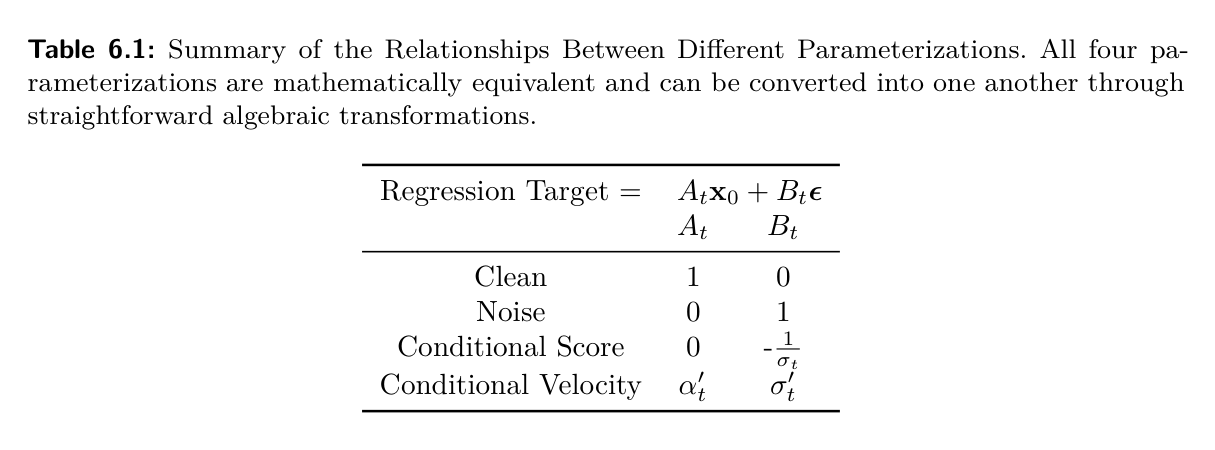
\includegraphics[width=0.95\textwidth,height=0.72\textheight,keepaspectratio]{table-6-1.png}
\end{frame}
%=============================================
\asmain
\begin{frame}{表6.1の読み方}
    回帰ターゲットは常に
    \[
        A_t\vx_0+B_t\veps
    \]
    \renewcommand{\arraystretch}{1.15}
    \begin{tabular}{lll}
        \hline
        予測型 & $A_t$ & $B_t$ \\
        \hline
        Clean & $1$ & $0$ \\
        Noise & $0$ & $1$ \\
        Conditional Score & $0$ & $-\sigma_t^{-1}$ \\
        Conditional Velocity & $\alpha_t'$ & $\sigma_t'$ \\
        \hline
    \end{tabular}
    \vspace{0.4em}
    \begin{exampleblock}{含意}
        4パラメータ化は代数的に相互変換できる（後の式6.3.1）。
    \end{exampleblock}
\end{frame}
%=============================================
\asmain
\begin{frame}{マッチした予測と損失}
    式(6.2.5)の標準は、ネット出力と損失の予測型を一致させる：
    \begin{itemize}
        \item $x$-prediction $\leftrightarrow$ ターゲット$\vx_0$
        \item $v$-prediction $\leftrightarrow$ ターゲット$\alpha_t'\vx_0+\sigma_t'\veps$
    \end{itemize}
    \begin{block}{オラクル情報}
        4予測型は同じオラクル情報を符号化し、相互変換できる（式6.3.1）。
    \end{block}
\end{frame}
%=============================================
\asmain
\begin{frame}{予測と損失をずらす場合}
    ネットが直接出す量と、損失で測る量は分離できる。\\
    まず式(6.3.1)で変換し、変換先のターゲットと比較する。
    \begin{block}{例：標準線形$\vx_t=(1-t)\vx_0+t\veps$}
        ネットが$x_\phi$を出すとき、速度へ変換すると
        \[
            \bm{v}_\phi=\frac{\vx_t-x_\phi}{t},
            \qquad
            \bm{v}_t=\frac{\vx_t-\vx_0}{t}
        \]
        よって
        \[
            \|\bm{v}_\phi-\bm{v}_t\|_{2}^{2}
            =
            t^{-2}\|x_\phi-\vx_0\|_{2}^{2}.
        \]
    \end{block}
\end{frame}
%=============================================
\asmain
\begin{frame}{ずらし損失＝追加の時間重み}
    ネット出力をcleanに固定したままvelocity損失を使うのは、\\
    clean損失に時間依存重み$t^{-2}$を掛けたものと厳密同値。
    \begin{itemize}
        \item 一般アフィン＋他予測型の関係は後の式(6.3.6)
        \item 式(6.2.5)は、断りがなければ「マッチした」場合を指す
    \end{itemize}
    \begin{alertblock}{ネットが直接予測する量の追加効果}
        オラクルは代数変換できても、有限ネットは別関数を表現する。\\
        出力スケールとパラメータ勾配が変わる$\Rightarrow$最適化に効く。
    \end{alertblock}
\end{frame}
%=============================================
\section{(C)(D) 時間分布と重み}
\asmain
\begin{frame}{区切り：(C)(D) 時間分布と重み}
    \tableofcontents[currentsection]
\end{frame}
%=============================================
\asmain
\begin{frame}{固定時刻の回帰損失}
    便宜上、固定$t$の回帰損失を
    \[
        L_t(\phi)
        :=
        \mathbb{E}_{\vx_0,\veps}
        \bigl\|
        \mathrm{NN}_\phi(\vx_t,t)
        -
        (A_t\vx_0+B_t\veps)
        \bigr\|_{2}^{2},
        \quad
        \vx_t=\alpha_t\vx_0+\sigma_t\veps
    \]
    と書くと、式(6.2.5)は
    \[
        L(\phi)
        =
        \mathbb{E}_{t\sim p_{\mathrm{time}}}
        \bigl[\omega(t)\,L_t(\phi)\bigr].
    \]
\end{frame}
%=============================================
\asmain
\begin{frame}{(D) $p_{\mathrm{time}}$：目的を変えるか推定を変えるか}
    補正なしで時刻を偏ってサンプルすると、その時刻の重みも増える。\\
    期待損失のレベルでは、積$p_{\mathrm{time}}(t)\omega(t)$だけが効く。
    \vspace{0.4em}
    一方、目的を固定したまま提案$q_{\mathrm{time}}$から引き、
    \[
        L(\phi)
        =
        \mathbb{E}_{t\sim q_{\mathrm{time}}}
        \Bigl[
        \frac{p_{\mathrm{time}}(t)}{q_{\mathrm{time}}(t)}\,
        \omega(t)\,L_t(\phi)
        \Bigr]
    \]
    と補正すれば（importance sampling）、目的は不変で推定分散だけが変わる。
\end{frame}
%=============================================
\asmain
\begin{frame}{区別の標語}
    \[
        \begin{aligned}
        p_{\mathrm{time}}\text{を目的で変える}
        &\Longrightarrow
        \text{異なる重み、異なる目的}
        \\
        q_{\mathrm{time}}+\text{IS補正}
        &\Longrightarrow
        \text{同じ目的、異なる推定器}
        \end{aligned}
    \]
    \begin{itemize}
        \item 時間サンプリングと損失重みは概念的に分けておく
        \item 一様サンプリングでは密度が定数倍なので区別が見えにくい
        \item 非一様では「目的の定義か、ただの提案分布か」を明示する
    \end{itemize}
\end{frame}
%=============================================
\asmain
\begin{frame}{実務での現れ方}
    \begin{itemize}
        \item \textbf{ScoreFlow}：固定の尤度重み目的に対しISで分散低減
        \item \textbf{VDM}：ノイズレベル座標で目的を固定すると、\\
        スケジュールがIS分布のように振る舞う
        \item \textbf{EDM}：ノイズレベル上の非一様訓練分布と、\\
        別の損失重みを両方指定。実効重みは両者の積
    \end{itemize}
\end{frame}
%=============================================
\asmain
\begin{frame}{(C) 時間重み$\omega(t)$}
    固定$p_{\mathrm{time}}$の下で、$\omega(t)$が各時刻の相対寄与を決める。\\
    実効重みは$p_{\mathrm{time}}(t)\omega(t)$。
    \begin{itemize}
        \item 基線：一様時間＋$\omega(t)\equiv 1$（簡易$\veps$-pred、FM/RF）
        \item 尤度重み：スコア目的で$\omega(t)=g^{2}(t)$は、\\
        適当な正則性の下で負対数尤度の上界（Song et al., 2021）
        \item SNR依存重み：ノイズレベル間の強調を再配分
    \end{itemize}
\end{frame}
%=============================================
\assuppl
\begin{frame}{\supplmark：log-SNRと単調重み}
    腐敗度の座標としてlog-SNR
    \[
        \Lambda_t
        :=
        \log\frac{\alpha_t^{2}}{\sigma_t^{2}}
    \]
    を用いる（半log-SNR $\lambda_t=\tfrac12\Lambda_t$は第9章）。\\
    $\Lambda_t$はノイズが増えるほど減少する。
    \begin{exampleblock}{Kingma and Gao (2023)}
        共通予測パラメータ化の下で、有効重み$w(\Lambda)$が$\Lambda$について\\
        非増加なら、重み付き拡散目的は（$\phi$独立項を除き）\\
        ガウス摂動データ上の平均負ELBOとして書ける。
    \end{exampleblock}
\end{frame}
%=============================================
\assuppl
\begin{frame}{\supplmark：ELBO-with-augmentationの直観}
    \begin{itemize}
        \item 単調重みは「ただ一部のノイズを強調する」以上の意味をもつ
        \item 異なる腐敗強度での変分訓練を平均している、と読める
        \item 詳細は脚注の$\frac{d}{dt}L(t;\vx_0)$と部分積分の議論（論文本文）
    \end{itemize}
    \begin{block}{ゼミでの扱い}
        ここでは解釈の存在を押さえる。\\
        導出の細部は必要に応じて原論文へ。
    \end{block}
\end{frame}
%=============================================
\section{再パラメータ化と最適化}
\asmain
\begin{frame}{区切り：再パラメータ化と最適化}
    \tableofcontents[currentsection]
\end{frame}
%=============================================
\asmain
\begin{frame}{何が「同じ」で、何が「違う」か}
    \renewcommand{\arraystretch}{1.2}
    \begin{tabular}{p{0.42\textwidth}p{0.48\textwidth}}
        \hline
        主に再パラメータ化 & 最適化に効き得る \\
        \hline
        アフィン日程の時間／空間変換
            & ネットが直接予測する量の選択 \\
        オラクル予測の代数変換
            & 損失の予測型（実効時間重み） \\
        IS補正付きの提案$q_{\mathrm{time}}$
            & $p_{\mathrm{time}}$や$\omega(t)$の変更 \\
        \hline
    \end{tabular}
    \vspace{0.5em}
    \begin{alertblock}{教訓}
        数学的同値でも、有限ネット＋SGDでは挙動が変わり得る。
    \end{alertblock}
\end{frame}
%=============================================
\asmain
\begin{frame}{結論（6.2のメッセージ）}
    見た目の違う設計の多くは、\\
    「ノイズレベル上の実効重みをどう形作るか」として理解できる。
    \begin{itemize}
        \item 実効重みは最適化地形に影響する
        \item 単調重みなど特殊例では変分解釈も持つ
        \item 6.3では、予測・損失・アフィン流の同値をもっと精密に述べる
    \end{itemize}
\end{frame}
%=============================================
\section{まとめ}
\asmain
\begin{frame}{区切り：6.2のまとめ}
    \tableofcontents[currentsection]
\end{frame}
%=============================================
\asmain
\begin{frame}{6.2 全体のまとめ}
    \begin{enumerate}
        \item \textbf{四予測}
        $x$／$\veps$／$s$／$\bm{v}$はいずれも$\vx_t$条件付き期待
        \item \textbf{テンプレート}
        式(6.2.5)：$p_{\mathrm{time}}$、$\omega(t)$、ターゲット$A_t\vx_0+B_t\veps$
        \item \textbf{表6.1}
        $(A_t,B_t)$が予測型を決める；相互変換可能
        \item \textbf{設計の分解}
        スケジュール／予測／重み／時間分布を分けて考える
        \item \textbf{同値の注意}
        再パラメータ化と、最適化に効く変更を混同しない
    \end{enumerate}
\end{frame}
%=============================================
\asmain
\begin{frame}{6.2 全体のまとめ：一本の流れ}
    \begin{block}{今日の道筋}
        条件付け原理
        $\;\to\;$
        4予測型
        $\;\to\;$
        テンプレート損失
        $\;\to\;$
        (A)--(D)の設計空間
    \end{block}
    \begin{block}{核心}
        拡散の訓練は「どの量を、どのノイズレベルで、どれだけ強調して回帰するか」。\\
        同値変換と実効重みの変化を分けて読む。
    \end{block}
    \begin{block}{次へ（6.3）}
        予測・目的・アフィン前向き過程の同値を精密化する。
    \end{block}
\end{frame}
